\paragraph{}Esta es la página principal o de inicio de la aplicación web $\mu$Search para el administrador de la misma. A esta página de inicio, el administrador será siempre redirigido cuando pulse en cualquiera de los dos logotipos de la cabecera de la página.

\paragraph{}Se le muestra al administrador un mensaje de bienvenida y una breve descripción las funcionalidades que tiene disponibles como administrador de la aplicación web.

\begin{figure}[h!]
	\centering
	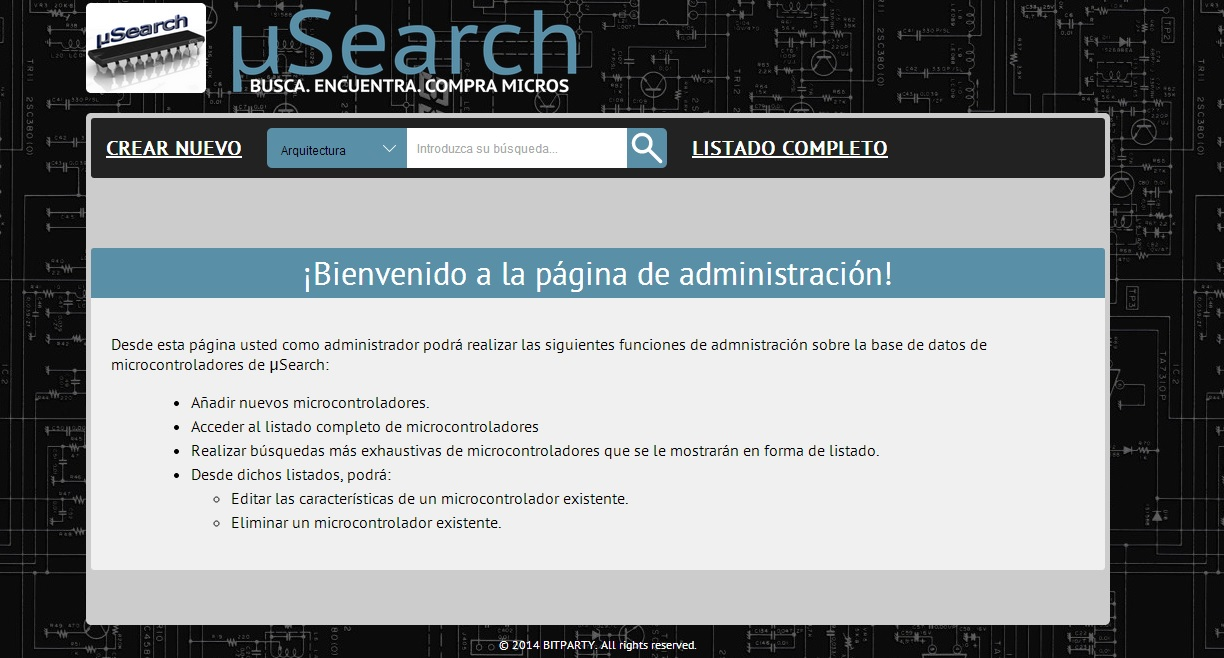
\includegraphics[width=0.75\textwidth]{img/principal_admin}
	\caption{Página principal de administración.}
	\label{fig:principal_admin}
\end{figure}

Desde esta página, a través de los iconos situados en la cabecera debajo de los logotipos de la web, el administrador puede acceder a:
\begin{itemize}
	
	\item \textbf{Crear Nuevo:} Pulsando sobre este botón el administrador es redirigido a la página que le permitirá añadir un nuevo microcontrolador a la base de datos del catálogo electrónico.
	
	\item \textbf{Búsqueda:} Desde esta sección, el administrador puede realizar búsquedas sobre el catálogo de microcontroladores en base a cualquiera de las características de un microcontrolador (Arquitectura, Frecuencia, Flash, RAM). Simplemente se debe seleccionar una de las características de la lista despegable, introducir el texto a buscar y pulsar sobre el icono de búsqueda.
	El administrador será redirigido a una página donde se le mostrará el resultado de la búsqueda en forma de lista de microcontroladores.
	
	\item \textbf{Listado Completo:} Pulsando sobre este botón/icono el sistema redirige al administrador a la página en la que se listan todos los elementos disponibles en el catálogo de microcontroladores, con sus correspondientes características.
	
\end{itemize}